\section{Discussion with Practical Examples and Cases}
\label{sec:discussion}

\todo{OLD EVALUATION SECTION}

The new language has been evaluated through a prototype implementation that builds on 
the ASTRA~\cite{DBLP:conf/prima/CollierRL15} language. This prototype, which is compatible
with pure ASTRA code, is used to reimplement part of an existing solution for the Minority 
Game~\cite{moro2004minority}. Interpreter cycle timings are then captured to develop an initial
understanding of how the new language performs.

{\small
\begin{verbatim}
g-plan +!g() : c <: gc { 
  body {
    // main plan body goes here...
    a; b; !g1(); !!g2();
  }

  /* e-plans */
  rule +e1 : c1 { b1; }
  rule +e2 : c2 { b2; }
}
\end{verbatim}}

As can be seen in the  snippet of code above, the implementation of the {\aser} prototype is 
syntactically different to the examples provided in Section~\ref{sec:proposal}. This reflects 
the syntactic approach adopted in ASTRA. It does not impact the associated semantics.

\subsection{Minority Game}
\label{minority}
The Minority Game is a well-known model for evaluating collective behaviour of agents competing 
for finite resources~\cite{moro2004minority}. In a nutshell, the game involves an odd number of
agents competing for a resource over a series of rounds. For a round, each agent makes a binary
decision (yes/no). At the end of the round, the bids are counted, and the agents that are in the
minority win. The game has been applied mainly in the areas such as modelling financial markets 
\cite{challet2013minority} and traffic simulation \cite{chmura2004minority}.

To provide an initial evaluation of {\aser}, we adapt an existing ASTRA-based implementation of 
the Minority Game (MG). As is shown in Figure~\ref{fig:mgagents}, the implementation consists of
3 types of agent: the \emph{compere} agent, who is responsible for managing the game (starting 
rounds, evaluating bids, ...); the \emph{player} agent, who implements a set of MG strategies; 
and the \emph{main} agent, which is responsible for configuring the game (creating and configuring
the compere and player agents). Interaction between the Compere and the Players is through a shared 
game-board artifact.

\begin{figure}[!tbh]
\centering
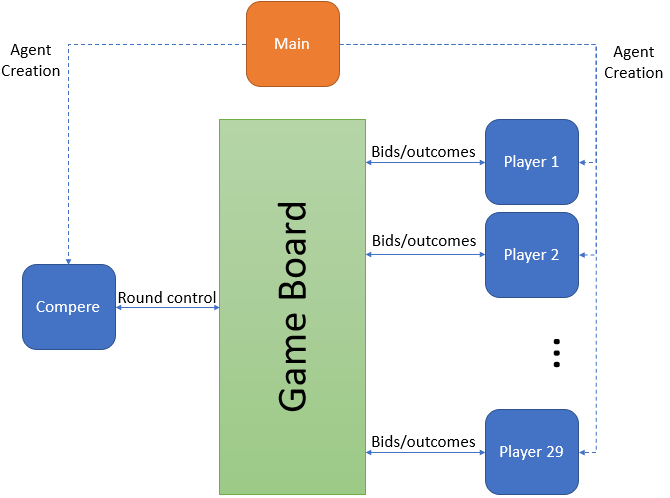
\includegraphics[height=2in, width=2.5in]{figs/mg.png}
\caption{Minority Game Agent Architecture}
\label{fig:mgagents}
\end{figure}

The existing implementation currently consists of 10 plans. Two of the plans are generic and are
used for configuration. Another plan implements the bidding behaviour, delegating to a 
\verb|!select_bid(...)| sub-goal that can be contextually selected based on the current strategy.
Of the remaining plans: four relate to the best play strategy; one relates to a random strategy;
and two relate to a sticky strategy.


In the {\aser} implementation, we reduce this to 3 g-plans --- one for each of the strategies --- 
and one traditional plan to handle initialization. The code below consists of the initialisation 
plan and a single g-plan representating the revised implementation of the best play strategy.

In the code below, variable \verb|A| represents the game board, which
is implemented as an ASTRA module~\cite{DBLP:conf/prima/CollierRL15}. Modules allow the developer to
create custom actions, sensors, (logical) terms, (logical) formulae,
and events. For example, \verb|A.join()| is a custom action to allow
the agent to join the game board; \verb|A.match(history, hist)| is a
custom term that returns the length of the longest common suffix of the
\verb|history| and \verb|hist| lists; and
\verb|$A.event(...)| is a custom event that is generated when the
Compere agent starts a new round.

The initialisation plan selects the game strategy to be employed by the player. This information
 is passed via the \verb|main(...)| goal; the ASTRA equivalent of a
 main method. When the interpreter handles
the event corresponding to this goal, it spawns a new intention to achieve the \verb|win(...)| 
goal (spawning is like forking in multi-processing and is denoted the double exclamation mark).

When the chosen strategy is \emph{bestplay}, the agent achieves the goal by selecting 
the \verb|!win("bestplay", ...)| g-plan. Upon adoption, the body of this plan is executed, which 
in this case creates a random set of strategies that are to be used by the agent to select its 
bid. This involves adopting the \verb|!setup_tactic()| subgoal which is handled by the first two 
rules within the g-plan. The start of a round is modelled through the custom event 
\verb|$A.event("play", [])|. The rule that is selected to handle this event chooses the best 
strategy from the set of strategies available to the agent. Finally, the end of a round is modelled 
through the custom event \verb|$A.event("winner", [int bid])|. The rule that is selected to handle 
this event updates the score for all strategies that lead to \verb|bid| being selected.

{\small
\begin{verbatim}
rule +!main([string strategy, list config]) {
  !!win(strategy, config); A.join();
}

g-plan +!win("bestplay", [int t, int h]) <: false {
  body { !setup_tactic(t); }

  rule +!setup_tactic(0) {}
  rule +!setup_tactic(int t2) {
    list hist = [];
			
    // construct a random history
    int i=0;
    while (i<h) {
      hist = hist + [M.randomInt() % 2];
      i++;
    }
    +strategy(t2, hist, M.randomInt() % 2);
    +score(t2, 0);
		
    !setup_tactic(t2-1);
  }
		
  rule $A.event("play", []) { 
    list history = A.results();
			
    int max_len = -1; int max_choice = -1;
    int max_score = -1;
    foreach (strategy(int s, list hist, int c) 
              & score(s, int sc)) {
      int len = A.match(history, hist);
      if ((len > max_len) | 
          ((len == max_len) & (max_score < sc))) {
        max_choice = c; max_score = sc;
        max_len = len;
      }
    }
    A.bid(max_choice);
  }

  rule $A.event("winner", [int bid]) {
    foreach (strategy(int s, list hist, bid) 
           & score(s, int sc)) {
      -+score(s, sc+1);
    }
  }
}
\end{verbatim}}

Some interesting observations from adapting the code were: (i) the compexity of the plan contexts 
were simplified when using g-plans because the g-plan itself provided some of the context; (ii) 
the number of arguments passed as parameters was reduced, again because the scope of the parameters 
of the g-plan was the plan body \emph{and} all of its sub-plans; (iii) the total number of rules 
under consideration on each iteration was significantly less because only the rules within an 
active g-plan were considered by the agent --- for example, in the original implementation, there 
was always at least one applicable \verb|+!select_bid()| plan per strategy, whilst in the new 
implementation only the plans related to the current strategy were applicable.

\subsection{Preliminary Analysis}
\label{performance}

We evaluate the prototype by comparing the {\aser} and ASTRA implementations. Initially,
we compared interpreter cycle execution time and the number of iterations based on a
single configuration of the MG with 29 players and 1000 rounds. For our results, we averaged
the values across all 29 players and repeated the experiment 5 times.

\begin{table}[]
\centering
\caption{Comparing ASTRA and {\aser}}
\label{comparison}
\begin{tabular}{lll}
                            & ASER    & ASTRA  \\
Cycle Time (ms)             & 0.0017  & 0.0036 \\
Cycles                      & 293,772 & 62,880 \\
Elapsed Execution Time (ms) & 495.22  & 229.29 \\
Unix (timed)                & 16s     & 15s   
\end{tabular}
\end{table}

Results of our initial comparison can be found in Table~\ref{comparison}. The difference
in the number of cycles is due primarily to the scheduling algorithm used by ASTRA, which
suspends agents that have no sensors (perceptors) and whose event and intention queues are empty.
The impact of this is that ASTRA is generally more efficient than {\aser}. Due to the small but 
consistent difference in performance between the unix timing of the two experiments, we then 
explored how increasing the number of rounds affected performance. Results for this are shown 
in Table~\ref{rounds}.

\begin{table}[]
\centering
\caption{ASTRA vs {\aser} Performance}
\label{rounds}
\begin{tabular}{llllll}
           & 1000   & 2000   & 3000   & 4000   & 10000   \\
ASER (s)   & 15.514 & 30.251 & 44.202 & 57.736 & 140.059 \\
ASTRA (s)  & 14.893 & 28.232 & 42.168 & 56.453 & 137.379 \\
Diff. (\%) & 4.2\%  & 6.8\%  & 4.8\%  & 2.3\%  & 2.0\%  
\end{tabular}
\end{table}

This second table shows that {\aser} has a small impact on performance, but it is 
almost linear in this case (ASTRA shows a performance improvement of between 2-6\%).

While this is not a thorough evaluation of {\aser}, it does hint that the use of
goal conditions does not significantly impact the performance of the language. It 
must also be noted that the prototype implementation is not as mature as the ASTRA
implementation --- interpreter optimisations could further reduce the difference 
in performance.

